\chapter{Analysis}

\section{Actors}

\begin{itemize}
    \item \textbf{Unregistered User}: A visitor who has not logged in on the platform.
    
    \item \textbf{Registered User}: A user who has created an account on the platform.
    
    \item \textbf{Manager}: A registered user with administrative privileges.
\end{itemize}

\section{Functional Requirements}

The system should provide the following features for each type of user:

\begin{itemize}
    \item \textbf{Browse Media Contents}.
    
    \item \textbf{Search and Filter Media Contents}:
    \begin{itemize}
        \item Find specific manga or anime by title.
        \item Utilize basic filtering options to refine the media content list.
    \end{itemize}
    
    \item \textbf{View Media Content Trends}.
    
    \item \textbf{View Media Content}:
    \begin{itemize}
        \item View limited information about each media content.
    \end{itemize} 
    
    \item \textbf{View Media Content Details}:
    \begin{itemize}
        \item View detailed information about each media content.
        \item View reviews and ratings for each media content.
        \item View number of likes for each media content.
    \end{itemize}
    
    \item \textbf{Browse Users}.
    
    \item \textbf{Search Users by Username}.
    
    \item \textbf{View User}:
    \begin{itemize}
        \item View limited information about each user.
    \end{itemize} 
    
    \item \textbf{View User Details}:
    \begin{itemize}
        \item View detailed information about each user.
        \item View anime and manga liked by the user.
        \item View followers and following of the user.
    \end{itemize}
\end{itemize}

\subsection*{Unregistered User}

\begin{itemize}
    \item \textbf{Register/Login}:
    \begin{itemize}
        \item Create a new account to access additional features.
        \item Use valid credentials (email and password) to log into the account.
    \end{itemize}
\end{itemize}

\subsection*{Registered User}

\begin{itemize}
    \item \textbf{Logout}.
    
    \item \textbf{Profile Management}:
    \begin{itemize}
        \item Edit and update personal information (e.g., profile picture, bio).
        \item Delete own profile.
    \end{itemize}
    
    \item \textbf{Like/Unlike Media Contents}.
    
    \item \textbf{Follow/Unfollow Users}.
    
    \item \textbf{Review Media Contents}:
    \begin{itemize}
        \item Add comment and rating to manga and anime.
        \item Edit/Delete own reviews.
    \end{itemize}
    
    \item \textbf{Advanced Recommendations}:
    \begin{itemize}
        \item Receive media content suggestions based on user interactions and personal information.
        \item Receive users suggestions based on user interactions.
    \end{itemize}
\end{itemize}

\subsection*{Manager}

\begin{itemize}
    \item \textbf{Logout}.
    
    \item \textbf{Analytics Dashboard}:
    \begin{itemize}
        \item View user analytics (distribution and app rating).
        \item View manga analytics (trends and average rating).
        \item View anime analytics (trends and average rating).
    \end{itemize}
    
    \item \textbf{Content Management}:
    \begin{itemize}
        \item Add new media content (manga and anime).
        \item Update/Remove existing media content.
    \end{itemize}
\end{itemize}

\section{Non Functional Requirements}

\subsection*{Performance}

\begin{itemize}
    \item \textbf{Response Time}: The system should have low latency, with pages loading within an acceptable timeframe.
    
    \item \textbf{Scalability}: The system should be able to handle an increasing number of users and data without significant degradation in performance.
    
    \item \textbf{Concurrency}: The application should support multiple users simultaneously without performance bottlenecks. For very high traffic scenarios, acceptable delays may be introduced.
    
    \item \textbf{Availability}: The system should be available 24/7, with minimal downtime for maintenance.
    
    \item \textbf{Replication}: The system should have data replication to ensure data availability and fault tolerance.
\end{itemize}

\subsection*{Security}

\begin{itemize}
    \item \textbf{Controlled User Operations}: Users should only be able to perform operations that they are authorized to do.
\end{itemize}

\subsection*{Data Integrity}

\begin{itemize}
    \item \textbf{Data Consistency}: The system should maintain data consistency across all components and databases.
\end{itemize}

\subsection*{User Interface}

\begin{itemize}
    \item \textbf{Responsiveness}: The user interface should be responsive, providing a consistent and seamless experience across various devices and screen sizes.
    
    \item \textbf{Intuitiveness}: The interface should be user-friendly, with clear navigation and easily understandable features.
\end{itemize}

\section{UML class diagram}

\begin{figure}[h]\label{uml class diagram}
    \centering
    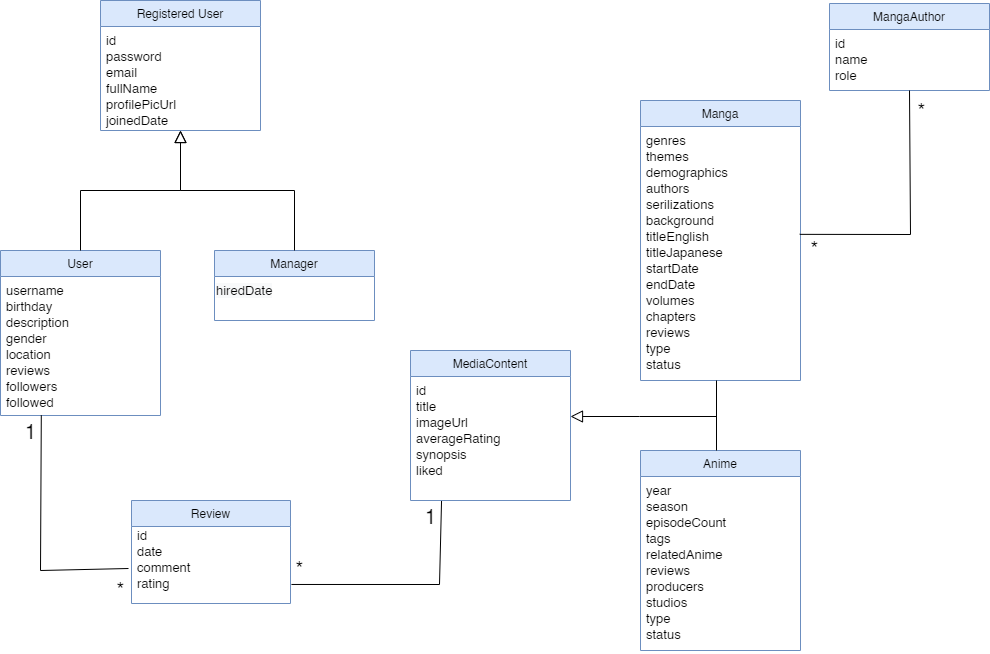
\includegraphics[width=\linewidth]{Media/Class Diagram.png}
\end{figure}

\newpage

\section{UML use case diagram}

\begin{figure}[h]\label{uml use case diagram}
    \centering
    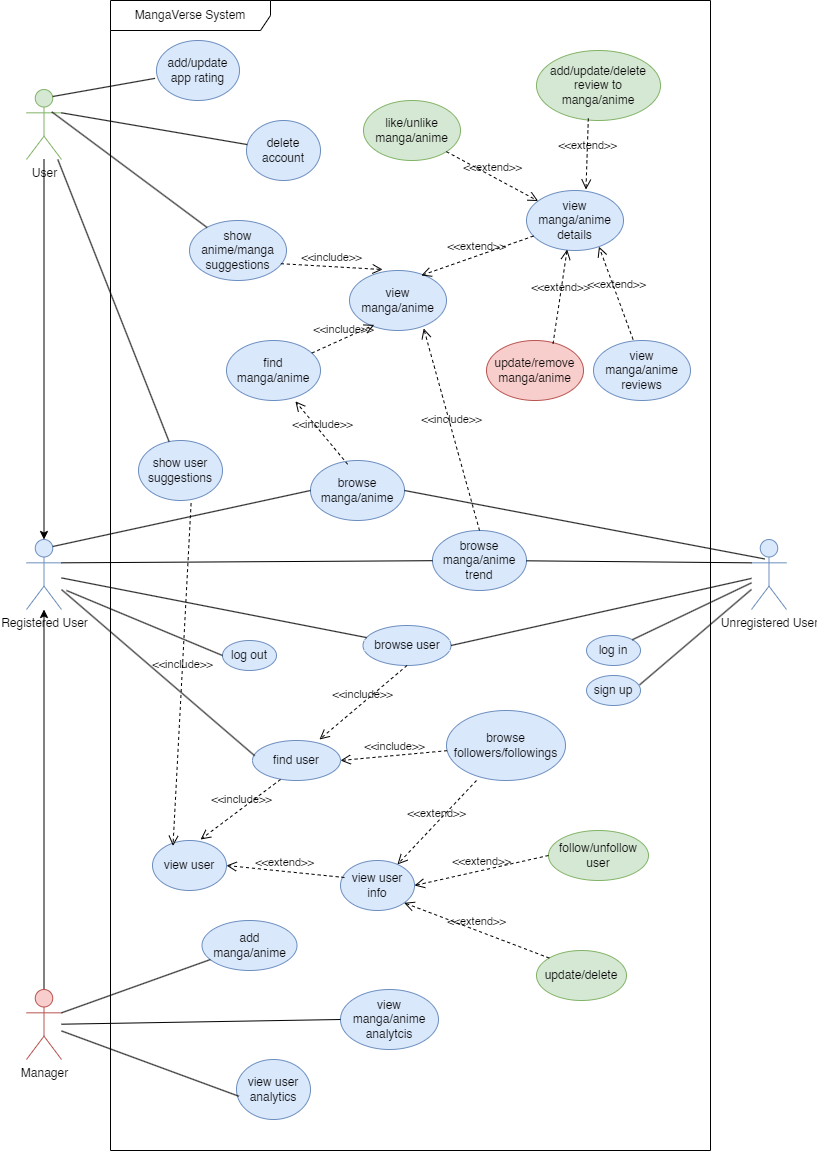
\includegraphics[width=0.85\textwidth]{Media/useCase.png}
\end{figure}

\newpage

\section{Data Modeling}

\subsection{Data Collection}

\textit{Sources:}
\href{https://myanimelist.net/}{myAnimeList.net}, 
\href{https://anilist.co/}{anilist.co},
\href{https://kitsu.io/}{kitsu.io},
\href{https://livechart.me/}{livechart.me}, \\
\href{https://anime-planet.com/}{anime-planet.com},
\href{https://notify.moe/}{notify.moe},
\href{https://anisearch.com/}{anisearch.com},
\href{https://anidb.net/}{anidb.net}.

\vspace{\baselineskip}

\textit{Description:} The datasets contain information about anime, manga, users, and scores. 
Anime and reviews are stored in separate CSV files. The manga dataset is collected from myAnimeList.net, 
scraped using the \href{https://myanimelist.net/apiconfig/references/api/v2}{Official API} and \href{https://docs.api.jikan.moe/}{Jikan API}.

\vspace{\baselineskip}

\textit{Variety:} Anime are collected from 8 different sources, manga from one source, 
and users/reviews from the same sources (myAnimeList and Anime-Planet). 
The data is structured across 4 CSV files and a JSON file.

\vspace{\baselineskip}

\textit{Volume:} $\sim$3 GB\@. The datasets contain approximately 10 million reviews, 40k anime entries, 70k manga entries, 
and 200k users.

\subsection{Data Cleaning and Preprocessing}

The data cleaning and preprocessing involved several steps to ensure consistency and usability of the datasets:

\begin{itemize}
    \item \textbf{Data Integration and Reduction}: Integrating anime, reviews, and user data from various sources 
    required dealing with non-unique IDs across datasets. To ensure proper integration, 
    new unique IDs were generated for each entity. Due to issues with data quality, 
    a significant number of users and their associated reviews were removed. This process resulted in a 
    refined dataset containing 10,000 users and 600,000 reviews.
 
    \item \textbf{Review Comment Generation}: Some sources lacked explicit comments for reviews. To address this, 
    a script was employed to generate generic comments based on the review ratings, ensuring completeness of the review dataset.
    
    \item \textbf{Synthetic Data Generation}: Many users did not have sufficient reviews for meaningful analytics. 
    Synthetic reviews were generated to supplement these users, enabling more robust analysis 
    of user interactions and content preferences.
    
    \item \textbf{Data Pruning}: Extraneous information about users, anime, and manga that were 
    not relevant to the project goals were removed to streamline the datasets.
    
    \item \textbf{Data Augmentation}: Essential user information such as email, password, and profile picture, 
    which were necessary for user management features, were added to the dataset.
    
    \item \textbf{Consistency Checks}: Before insertion into the Document DB collections, rigorous data consistency checks were conducted to 
    uphold accuracy and reliability. For instance, chronological consistency was enforced for fields such as the joined date, 
    ensuring it fell after the user's birthdate and before any related review dates. Additionally, user locations were validated 
    to ensure they mapped to valid countries. Upon insertion, Document DB's ids were utilized for entity linking and to maintain data integrity.

    \item \textbf{Graph Database Population}: Fake relationships were created, such as follow relationships between users and like relationships 
    between users and anime/manga, to populate the graph database.
\end{itemize}

\vspace{\baselineskip}

These steps were crucial in preparing the datasets for effective utilization within the MangaVerse platform, 
ensuring data quality and integrity across all components.

\vspace{\baselineskip}

Python was predominantly used for data preprocessing tasks, leveraging its flexibility and extensive libraries. 
Additionally, Java was employed for specific tasks such as adding and updating redundancies in the document database.